\subsubsection{VLAN de~\nameref{itm:vlan1}}
\par Para finalizar con las tareas requeridas por este trabajo en cuanto
a el \nameref{sec:escenario1}, se pasa a analizar la \textit{dataset} m\'as
grande de todos los capturados.

\par Como ya se describi\'o, la VLAN de \nameref{itm:vlan1} consta de una
gran variedad de diferentes dispositivos que cubren una extensa zona geogr\'afica.

\par Esta red originalmente era utilizada para tener una \'unica red para
todos los servicios y usuarios del organismo que n\'uclea al \textit{datacenter}.

\par As\'i pues, esperamos encontrarnos con una red con alta cantidad de 
paquetes ARP inundando el dominio de colisi\'on, y con una enorme cantidad
de distintas direcciones IP\footnote{La red en cuesti\'on es una red
clase \textit{A}}.

\par Siguiendo con el orden establecido en los casos anteriores, comenzaremos
presentando los resultados de los c\'alculos de entrop\'ia de ambas fuentes,
m\'as las caracter\'isticas del \textit{dataset}:

\begin{table}[!h]
\centering
  \begin{tabular}{c c}
    Fuente de Datos & Entrop\'ia \\
    \hline\hline
    Direcci\'on Origen & 5.8538 \\
    Direcci\'on Destino &  9.45154 \\
    \hline\hline
    \#IPs de las Fuentes & 50\,733 \\
    \#Paquetes Capturados & 11\,265\,364 \\
    \hline
    \end{tabular}
  \bigskip
  \caption{Entrop\'ia VLAN \nameref{itm:vlan1}}
  \label{tab:vlan1_entropia}
\end{table}

\par Ni bien presentado estos datos, llama la atenci\'on que de est\'as fuentes
de informaci\'on, que intu\'imos por el conocimiento de la red que tenemos, que
ser\'a m\'as ca\'otica (y por lo tanto ser\'ia esperable encontrarnos con una
alta entrop\'ia), nos da valores similiares a las fuentes de informaci\'on
presentadas en las secciones anteriores\footnote{Aunque claramente estos valores
son superiores a los ya expuestos, se esperaba una diferencia a\'un m\'as amplia.}


\subsubsection*{\underline{VLAN \nameref{itm:vlan1}: Fuente Origen}}\label{subsubsec:vlan1_src}
\par Se incluye a continuaci\'on las probabilidades por s\'imbolo de la fuente de direcci\'on
origne en la figura \ref{fig:vlan1_src_prob_per90}

\begin{figure}[!ht]
    \centering
    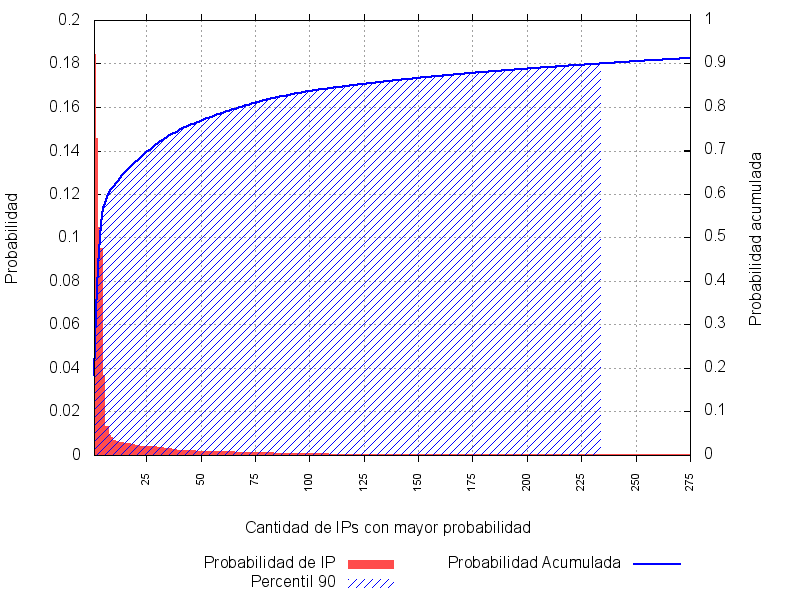
\includegraphics[width=0.5\textwidth]{escenario_1/vlan1/vlan1_src_bars_percentile90}
    \caption{Probabilidades VLAN \nameref{itm:vlan1} - Fuente Origen}
    \label{fig:vlan1_src_prob_per90}
\end{figure}

\par Al igual que en los casos anteriores donde tuvimos una entrop\'ia alta, se observa
en el gr\'afico que el percentil 90 se encuentra contenido en un porcentaje muy peque\~no
del total de s\'imbolos/IPs que provee la fuente de informaci\'on. Si bien, pareciese
que 260 IPs es un n\'umero grande si tenemos en cuenta las cantidades que venimos
analizando, no hay que perder de vista que en esta fuente obtuvimos un total de
50\,733 s\'imbolos distintos (n\'umero que supera con creces los hasta ahora vistos).

\par Si nos concentramos en las primeras 25 IPs, observamos que el percentil de la probabilidad
es el 70, el cu\'al nos muestra a\'un m\'as claramente la concentraci\'on de la informaci\'on
en las IPs con mayor probabilidad. Con 260 IPs se tiene un 90\% de la probabilidad mientras
que con 70 (menos de un tercio) se acumula un 70\%.

\begin{figure}[!ht]
    \centering
    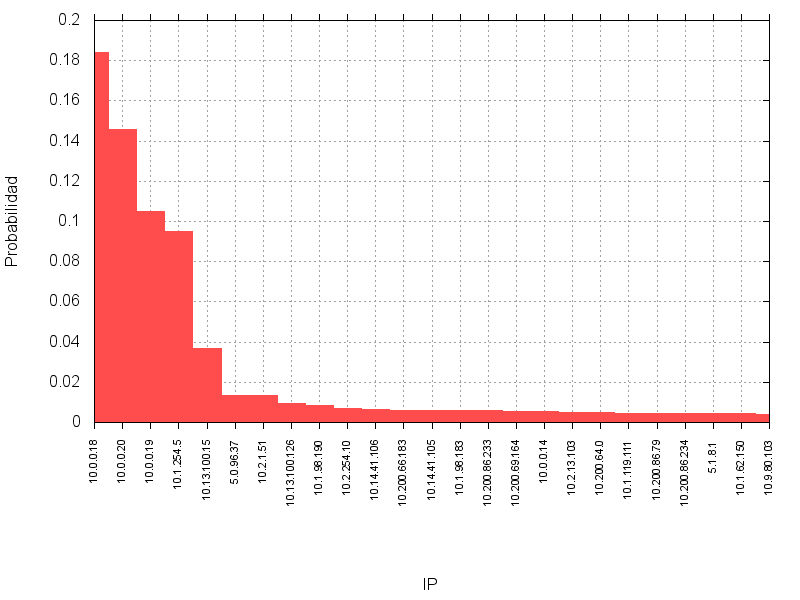
\includegraphics[width=0.5\textwidth]{escenario_1/vlan1/vlan1_src_probabilities_with_labels}
    \caption{IPs VLAN \nameref{itm:vlan1} - Fuente Origen}
    \label{fig:vlan1_src_prob_ips}
\end{figure}

\par Ya podemos entonces ir viendo que tendremos unos serios candidatos a nodos
importantes de la red a:

\begin{itemize}
    \item \textit{5.0.0.18}
    \item \textit{5.0.0.20}
    \item \textit{5.0.0.19}
    \item \textit{10.1.254.5}
    \item \textit{10.13.100.15}
    \item \textit{5.0.96.37}
\end{itemize}


\subsubsection*{\underline{VLAN \nameref{itm:vlan1}: Fuente Destino}}\label{subsubsec:vlan1_dst}
\par Sabiendo ya que para la fuente de destino tenemos una entrop\'ia de casi el
doble de la obtenida para la fuente de origen, es normal imaginar que nos
encontraremos cun un percentil 90 menos contenido. Si las matem\'aticas coinciden,
deber\'ia de ser de casi el doble de IPs.

\begin{figure}[!ht]
    \centering
    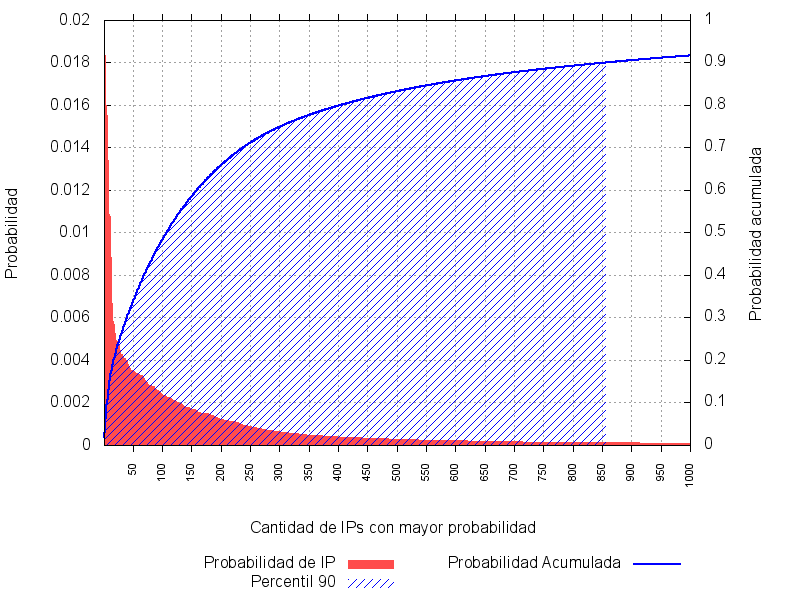
\includegraphics[width=0.5\textwidth]{escenario_1/vlan1/vlan1_dst_bars_percentile90}
    \caption{Probabilidades VLAN \nameref{itm:vlan1} - Fuente Destino}
    \label{fig:vlan1_dst_prob_per90}
\end{figure}

\par Efectivamente queda expl\'icito que se necesitan m\'as del doble de las IPs de mayor
probabilidad muestral para poder alcanzar el percentil 90. A\'un as\'i, con 850 IPs
segu\'imos muy lejos del total de s\'imbolos obtenidos de la fuente. Es decir,
la acumulaci\'on de la alta probabilidad en un numero reducido de IPs (aunque nominalmente
grande) nos da cierta informaci\'on sobre el comportamiento de la red, ya que la mayor
parte de la informaci\'on que da la fuente es reducida estad\'isticamente a un set
limitado\footnote{850 IPs contra 50\,733 es una diferencia nada desestimable.}.


\begin{table}[!h]
\centering
  \begin{tabular}{c c c c}
    Fuente& 
    Entrop\'ia & \begin{tabular}{@{}c@{}}Concentraci\'on \\ Percentil 90\end{tabular} 
    & \begin{tabular}{@{}c@{}}Concentraci\'on \\ Percentil 80\end{tabular}\\
    \hline\hline
    Origen & 5.8538 & 0.0045\% & 0.0012\%\\
    Destino & 9.45154 & 0.017\% & 0.008\%\\
    \hline\hline
    \end{tabular}
  \bigskip
  \caption{Concentraci\'on VLAN \nameref{itm:vlan1}}
  \label{tab:vlan1_concentracion}
\end{table}

\par Concentr\'emonos ahora en identificar posibles IPs importantes dentro de la red.
Para ello se presenta el siguiente gr\'afico con las 25 IPs con mayor probabilidad
de la fuente destino:

\begin{figure}[!ht]
    \centering
    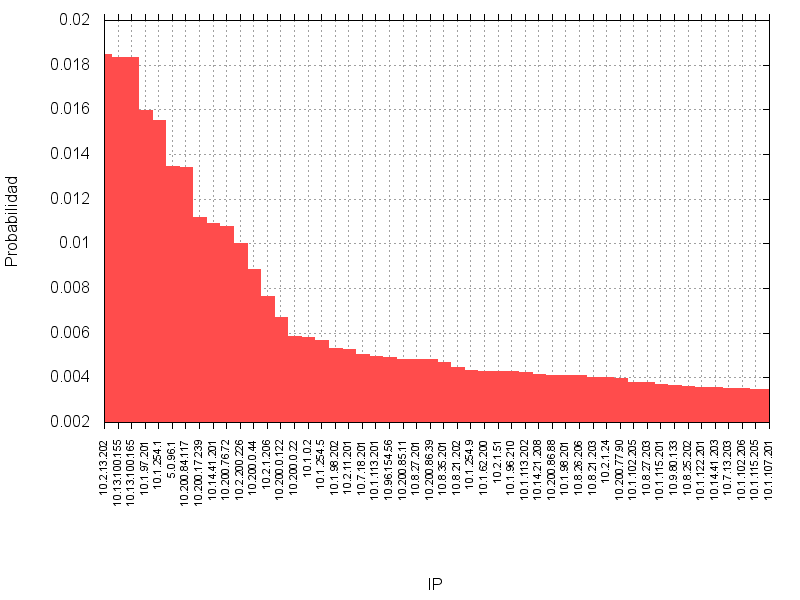
\includegraphics[width=0.5\textwidth]{escenario_1/vlan1/vlan1_dst_probabilities_with_labels}
    \caption{IPs VLAN \nameref{itm:vlan1} - Fuente Destino}
    \label{fig:vlan1_dst_prob_ips}
\end{figure}

\par Se puede observar aqu\'i que claramente los s\'imbolos que m\'as probabilidad muestral
acumulan son los primeros 15 de la figura \ref{fig:vlan1_dst_prob_ips}.


\subsubsection*{\underline{VLAN \nameref{itm:vlan1}: Ambas Fuentes}}\label{subsubsec:vlan1_src_dst}
\par A continuaci\'on se muestra un grafo con la informaci\'on tomada durante la semana de
captura de paquetes ARP. En el mismo, al igual que en casos anteriores, se
desestiman aquellos ejes que no tengan un peso superior a 1000 (es decir, que
no hayan sido env\'iados m\'as de 1000 veces con las mismas direcciones
origen y destino), ya que en el largo trayecto que se tomaron los datos
de la fuente de informaci\'on, dichos casos no aportan mucho a identificar
patrones constantes sobre el comportamiento de la red.

\par La figura \ref{fig:vlan1_grafo} nos muestra dicho grafo. Se ve que el mismo es muy grande
(como se esperaba) y deberemos analizarlo por partes para que se puedan sacar
conclusiones.

\par En un principio podemos observar que el grafo cuenta con 8 regiones bien delimitadas
a simple vista. Desde la componente no conexa que se ubica en la parte superior
derecha del grafo hasta las diferentes \textit{circunferencias} de nodos que parecen
tener un nodo importante, o al menos con muchos ejes, en el centro.

\par Curiosamente, estos nodos en el centro de estas \textit{circunferencias} suelen
tener ejes que los unan con los nodos que los rodean y ejes que los unen entre si. Pero,
si bien se ven algunas peticiones entre nodos centrales y nodos perif\'ericos de otras
circunferencias, esta no es la norma. Esto nos lleva ya a apuntar a que (sumado a los
colores de dichos nodos centrales), estos hosts representan o cumplen alguna funci\'on
destacable dentro de la red.

\begin{figure*}
    \centering
    \includegraphics[width=\textheight,angle=90]{img/graph/escenario_1/vlan1/vlan1_1000toEnd}
    \caption{Grafo VLAN \nameref{itm:vlan1}}
    \label{fig:vlan1_grafo}
\end{figure*}

\newpage
\par Comenzando a analizar la region disconexa, se puede ver detalladamente en la figura
~\ref{fig:vlan1_grafo_unconexed} que la mayor\'ia de las peticiones que ocurren son entre
pares de nodos (y siempre el mismo par ordenado). As\'i pues se ven ciertas conexiones
entre varios nodos hacia una misma direcci\'on, pero nunca en grandes cantidades y siempre
limitado a no m\'as de 5 direcciones origen. Esto parecer\'ia describir el comportamiento
que ocurre en ciertas oficinas de trabajo al compartir archivos por la red (o quiz\'as al
trabajar con los servicios de un servidor peque\~no).

\begin{figure}[!htb]
    \centering
    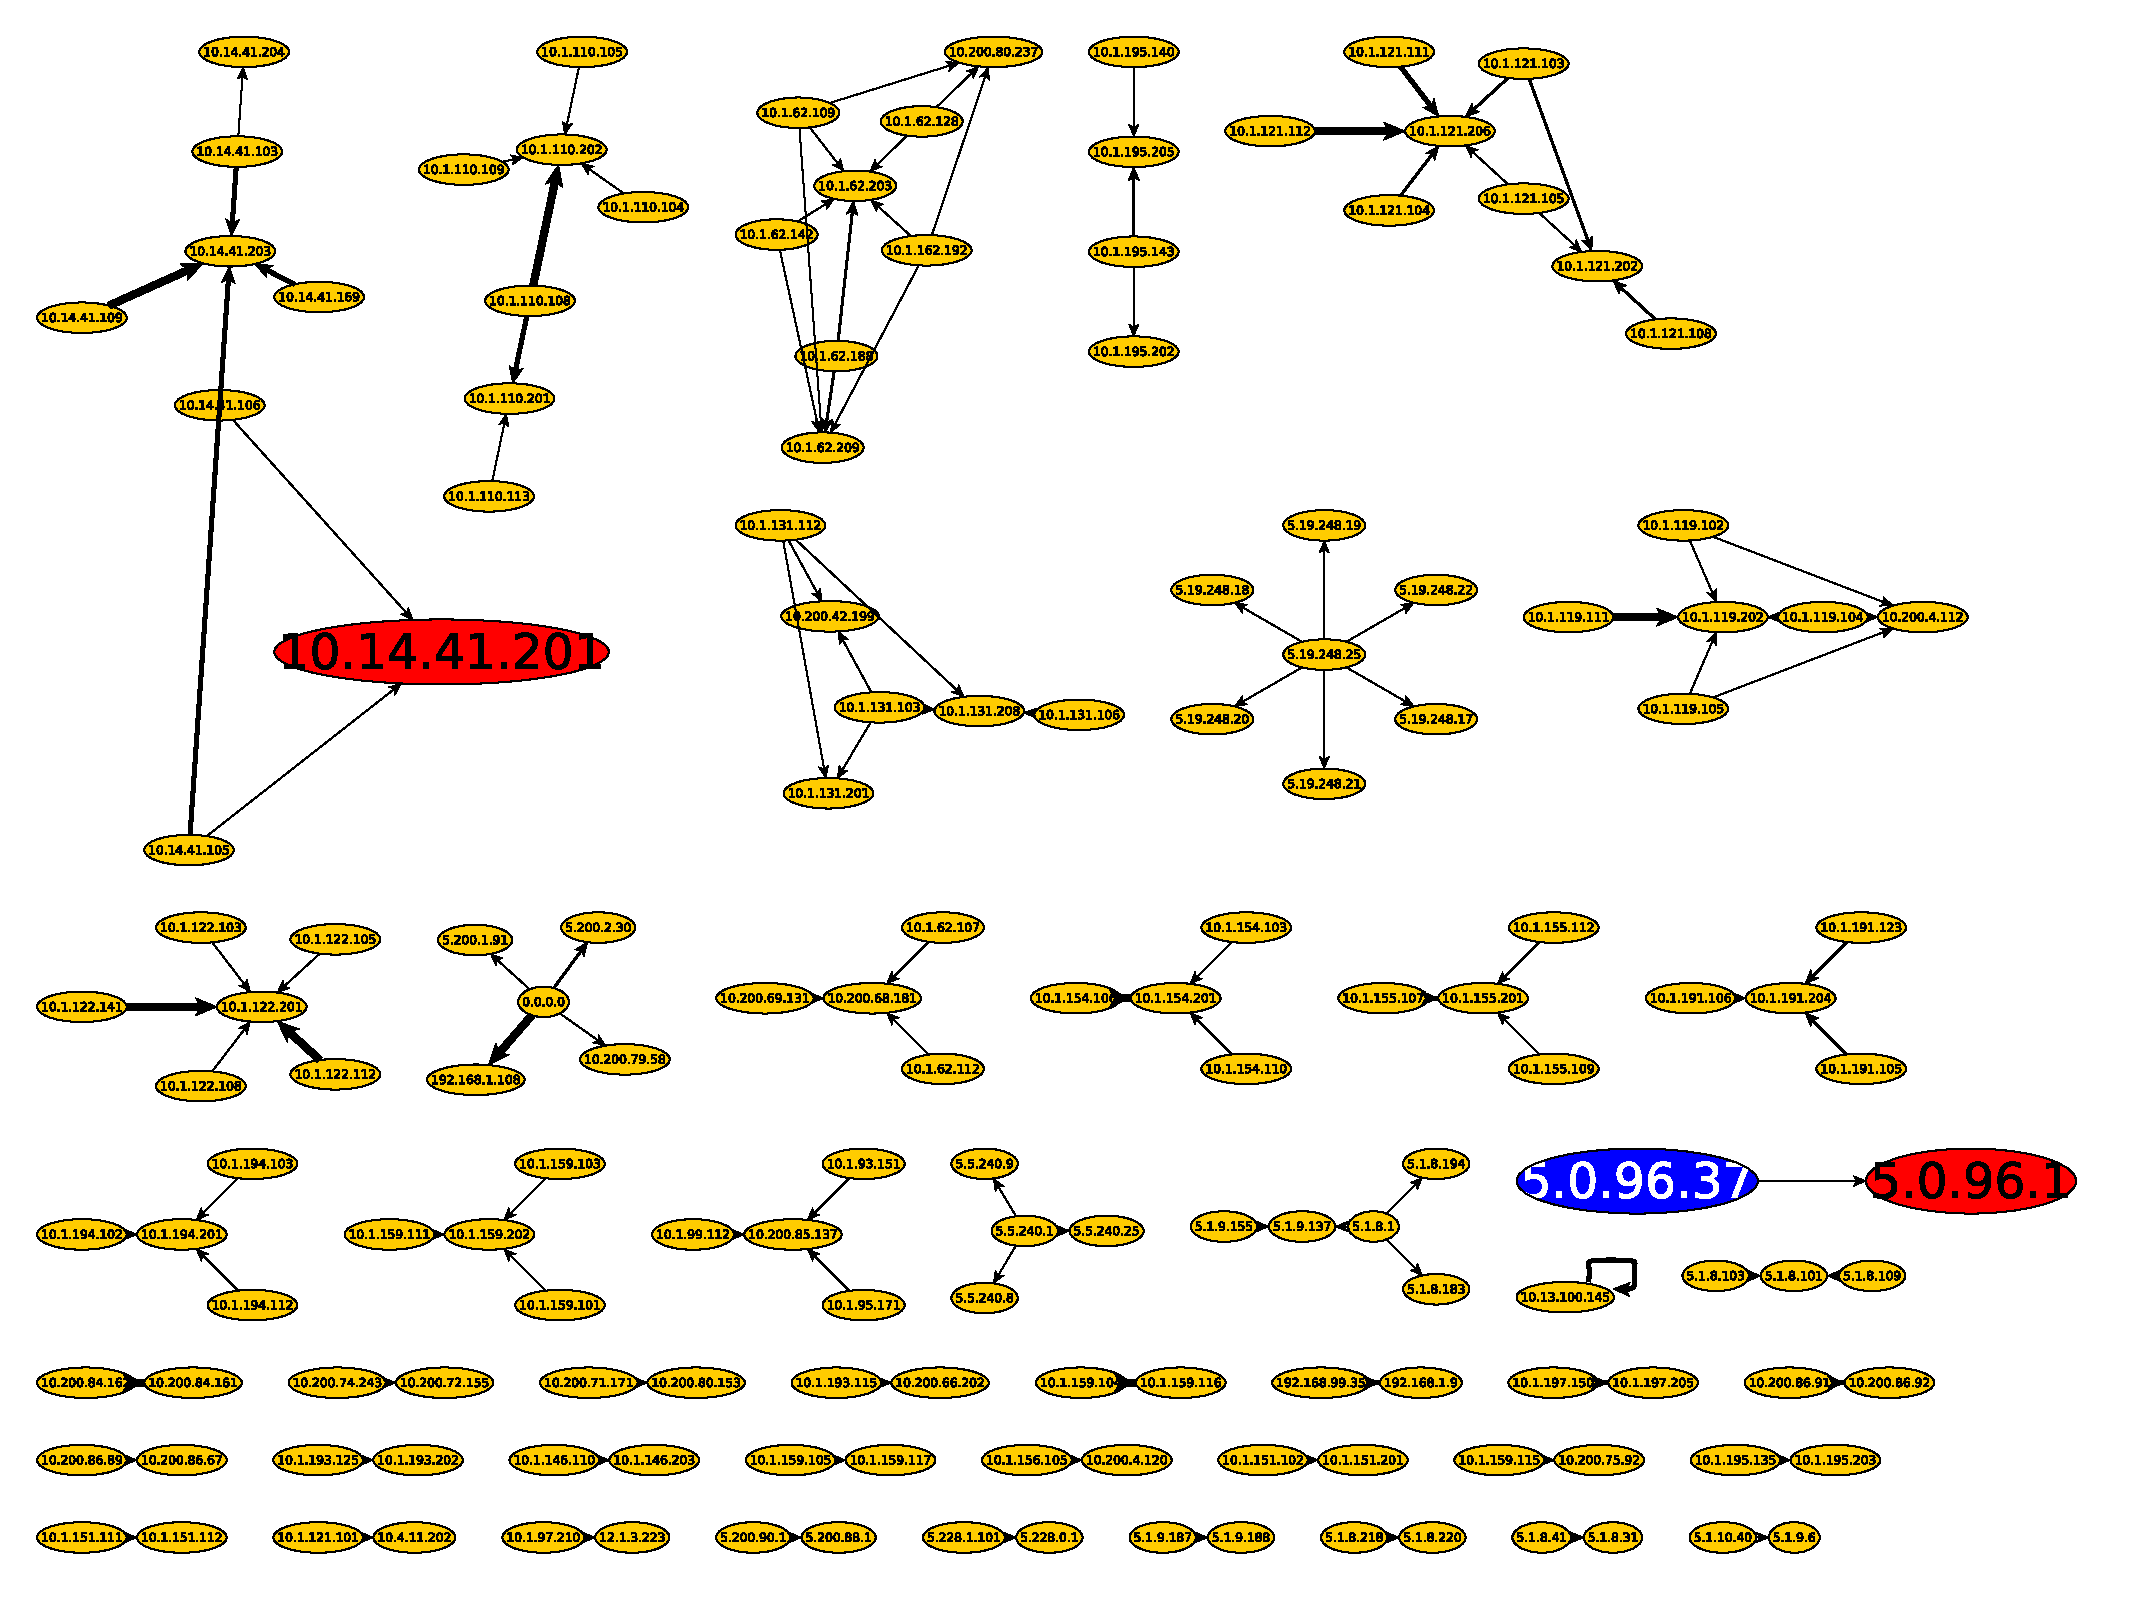
\includegraphics[width=0.5\textwidth]{img/graph/escenario_1/vlan1/vlan1_1000toEnd_unconexed}
    \caption{VLAN \nameref{itm:vlan1} - Componente Disconexo}
    \label{fig:vlan1_grafo_unconexed}
\end{figure}


\par Enfoc\'andonos sobre uno de los nodos ya se\~nalados en el inciso \ref{subsubsec:vlan1_src},
(figura \ref{fig:vlan1_grafo_10_0_0_19})
observamos que todos los paquetes constantes ARP tiene a la IP \textit{10.0.0.19} como direcci\'on
de origen. As\'i pues ser\'ia valido pensar que dicho host o se encuentra \textit{scanneando} la
red en busca siempre de las mismas IPs, o se trata de alg\'un servidor encargado de ofrecer
un servicio a un conjunto limitado de m\'aquinas de la red\footnote{NFS, Samba, DHCP, antivirus etc} o
quiz\'as de un equipo que se encuentra monitoreando a las otras direcciones.

\begin{figure}[!ht]
    \centering
    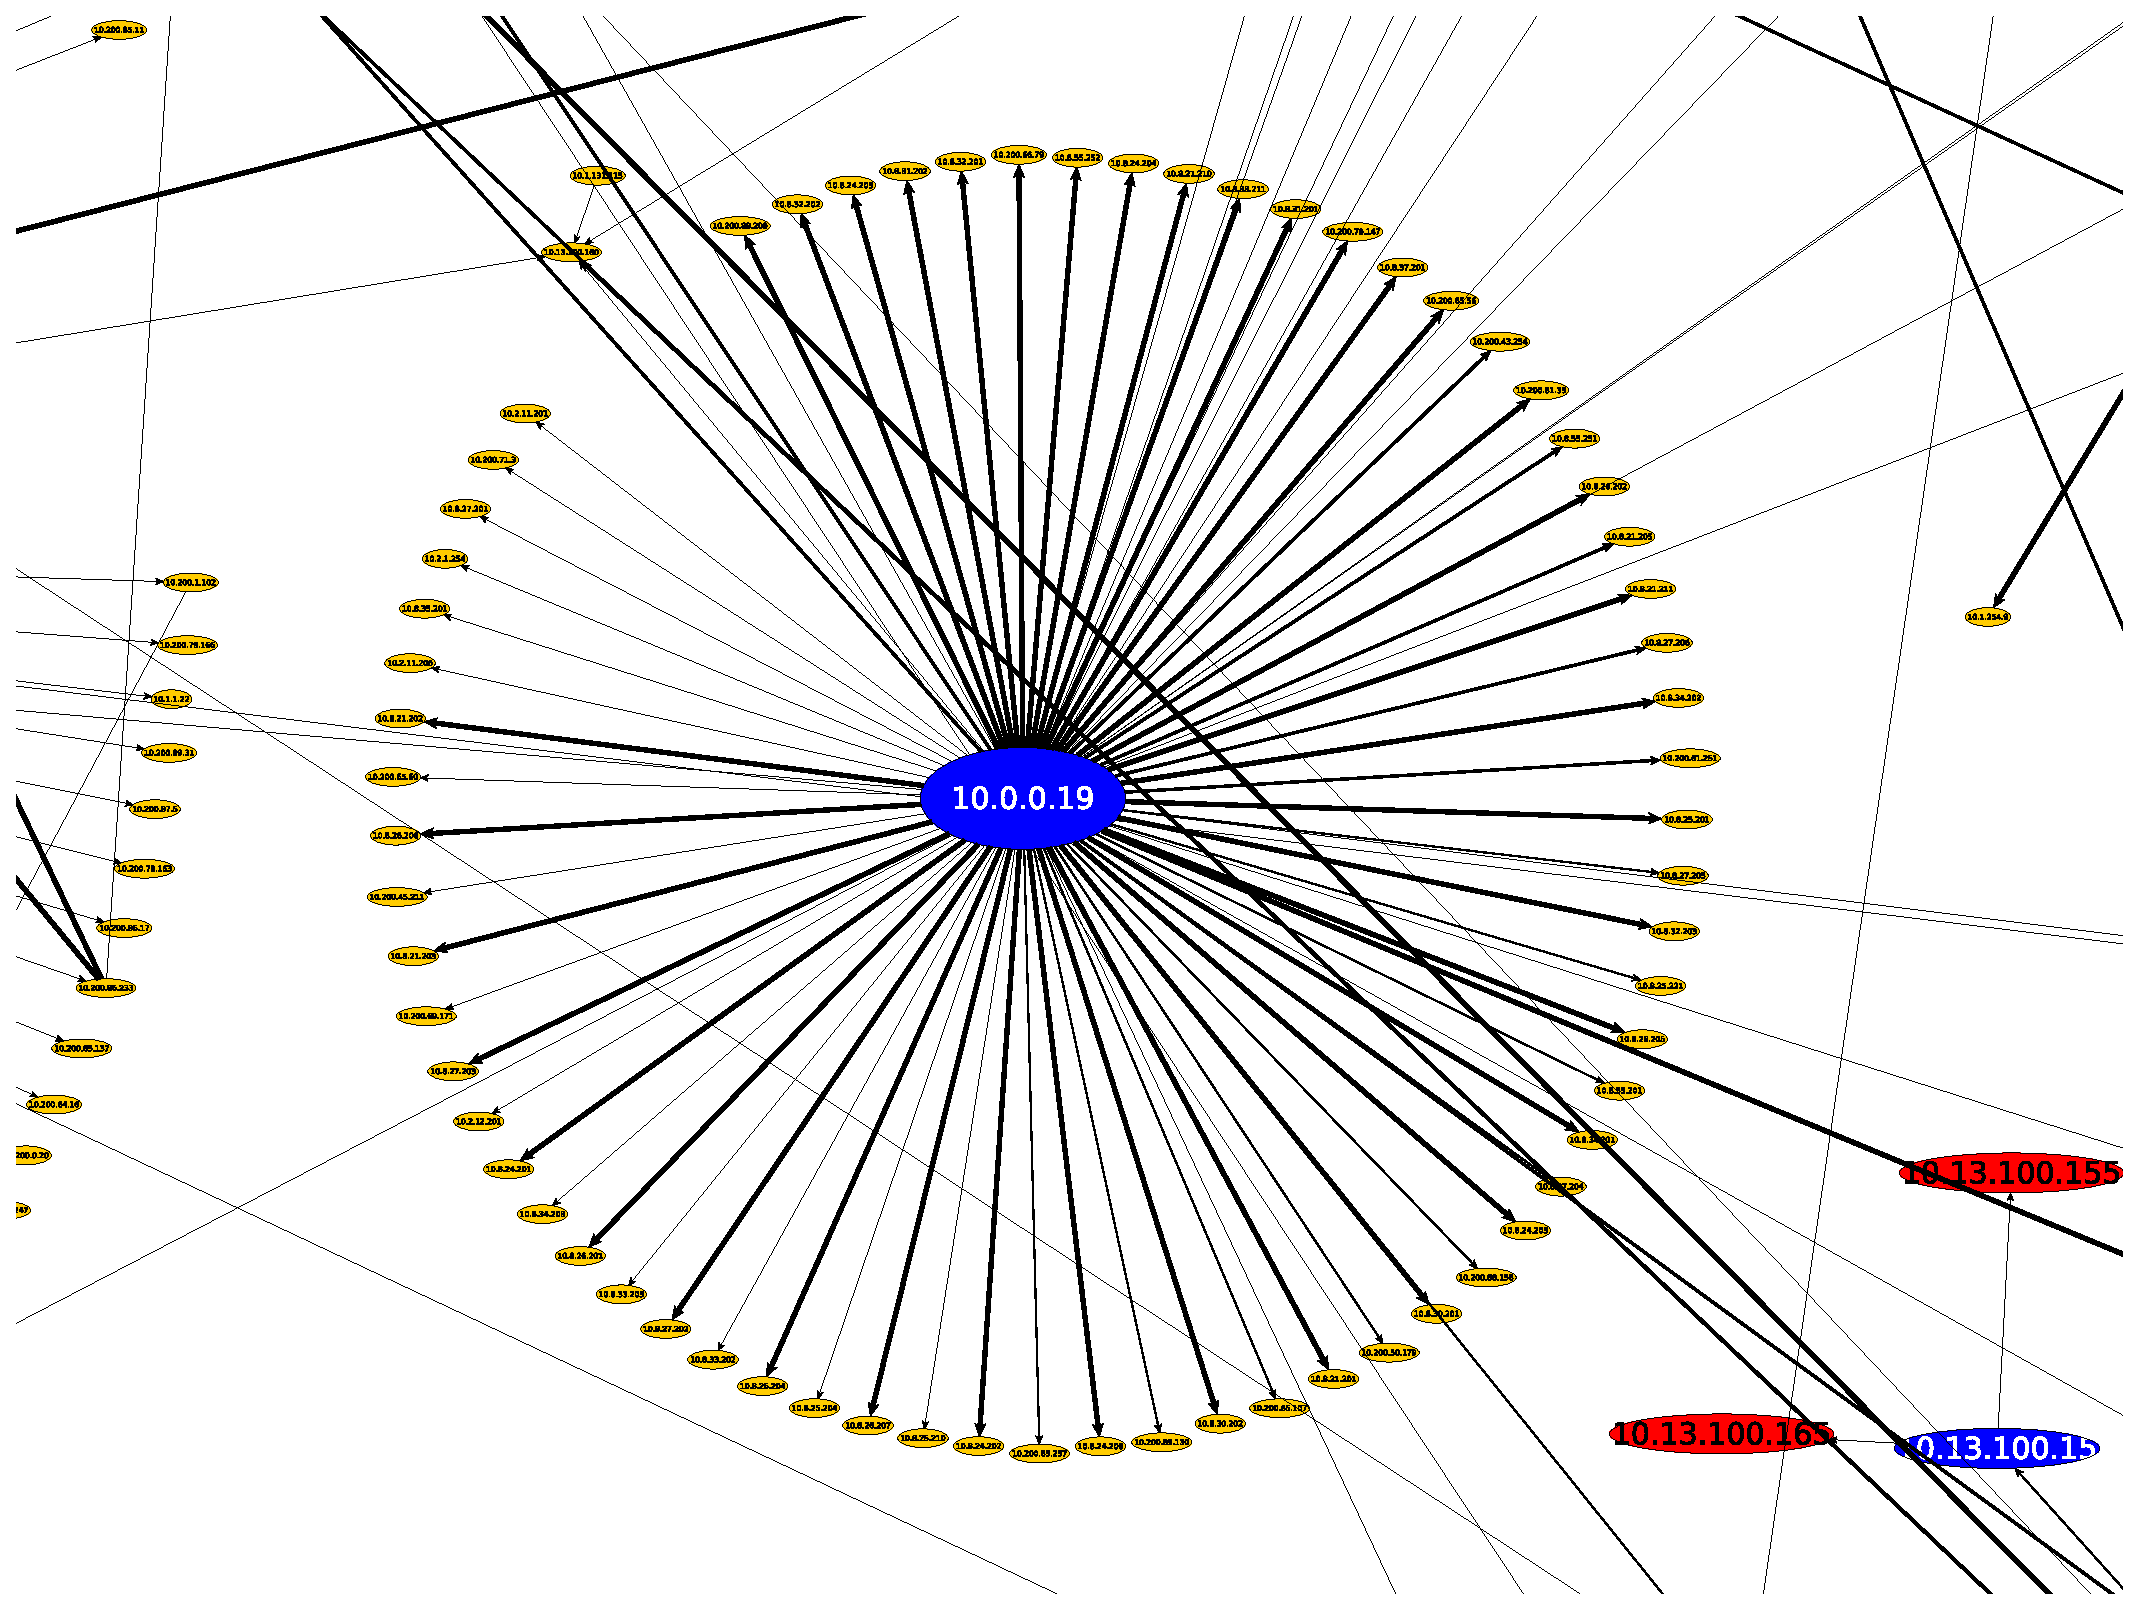
\includegraphics[width=0.5\textwidth]{img/graph/escenario_1/vlan1/vlan1_1000toEnd_10_0_0_19}
    \caption{VLAN \nameref{itm:vlan1} - 10.0.0.19}
    \label{fig:vlan1_grafo_10_0_0_19}
\end{figure}

\par Esto mismo aplica a las IPs \textit{10.0.0.18} y \textit{10.0.0.20}, tal como se puede ver
en las figuras \ref{fig:vlan1_grafo_10_0_0_18} y \ref{fig:vlan1_grafo_10_0_0_20}.

\begin{figure}[!ht]
    \centering
    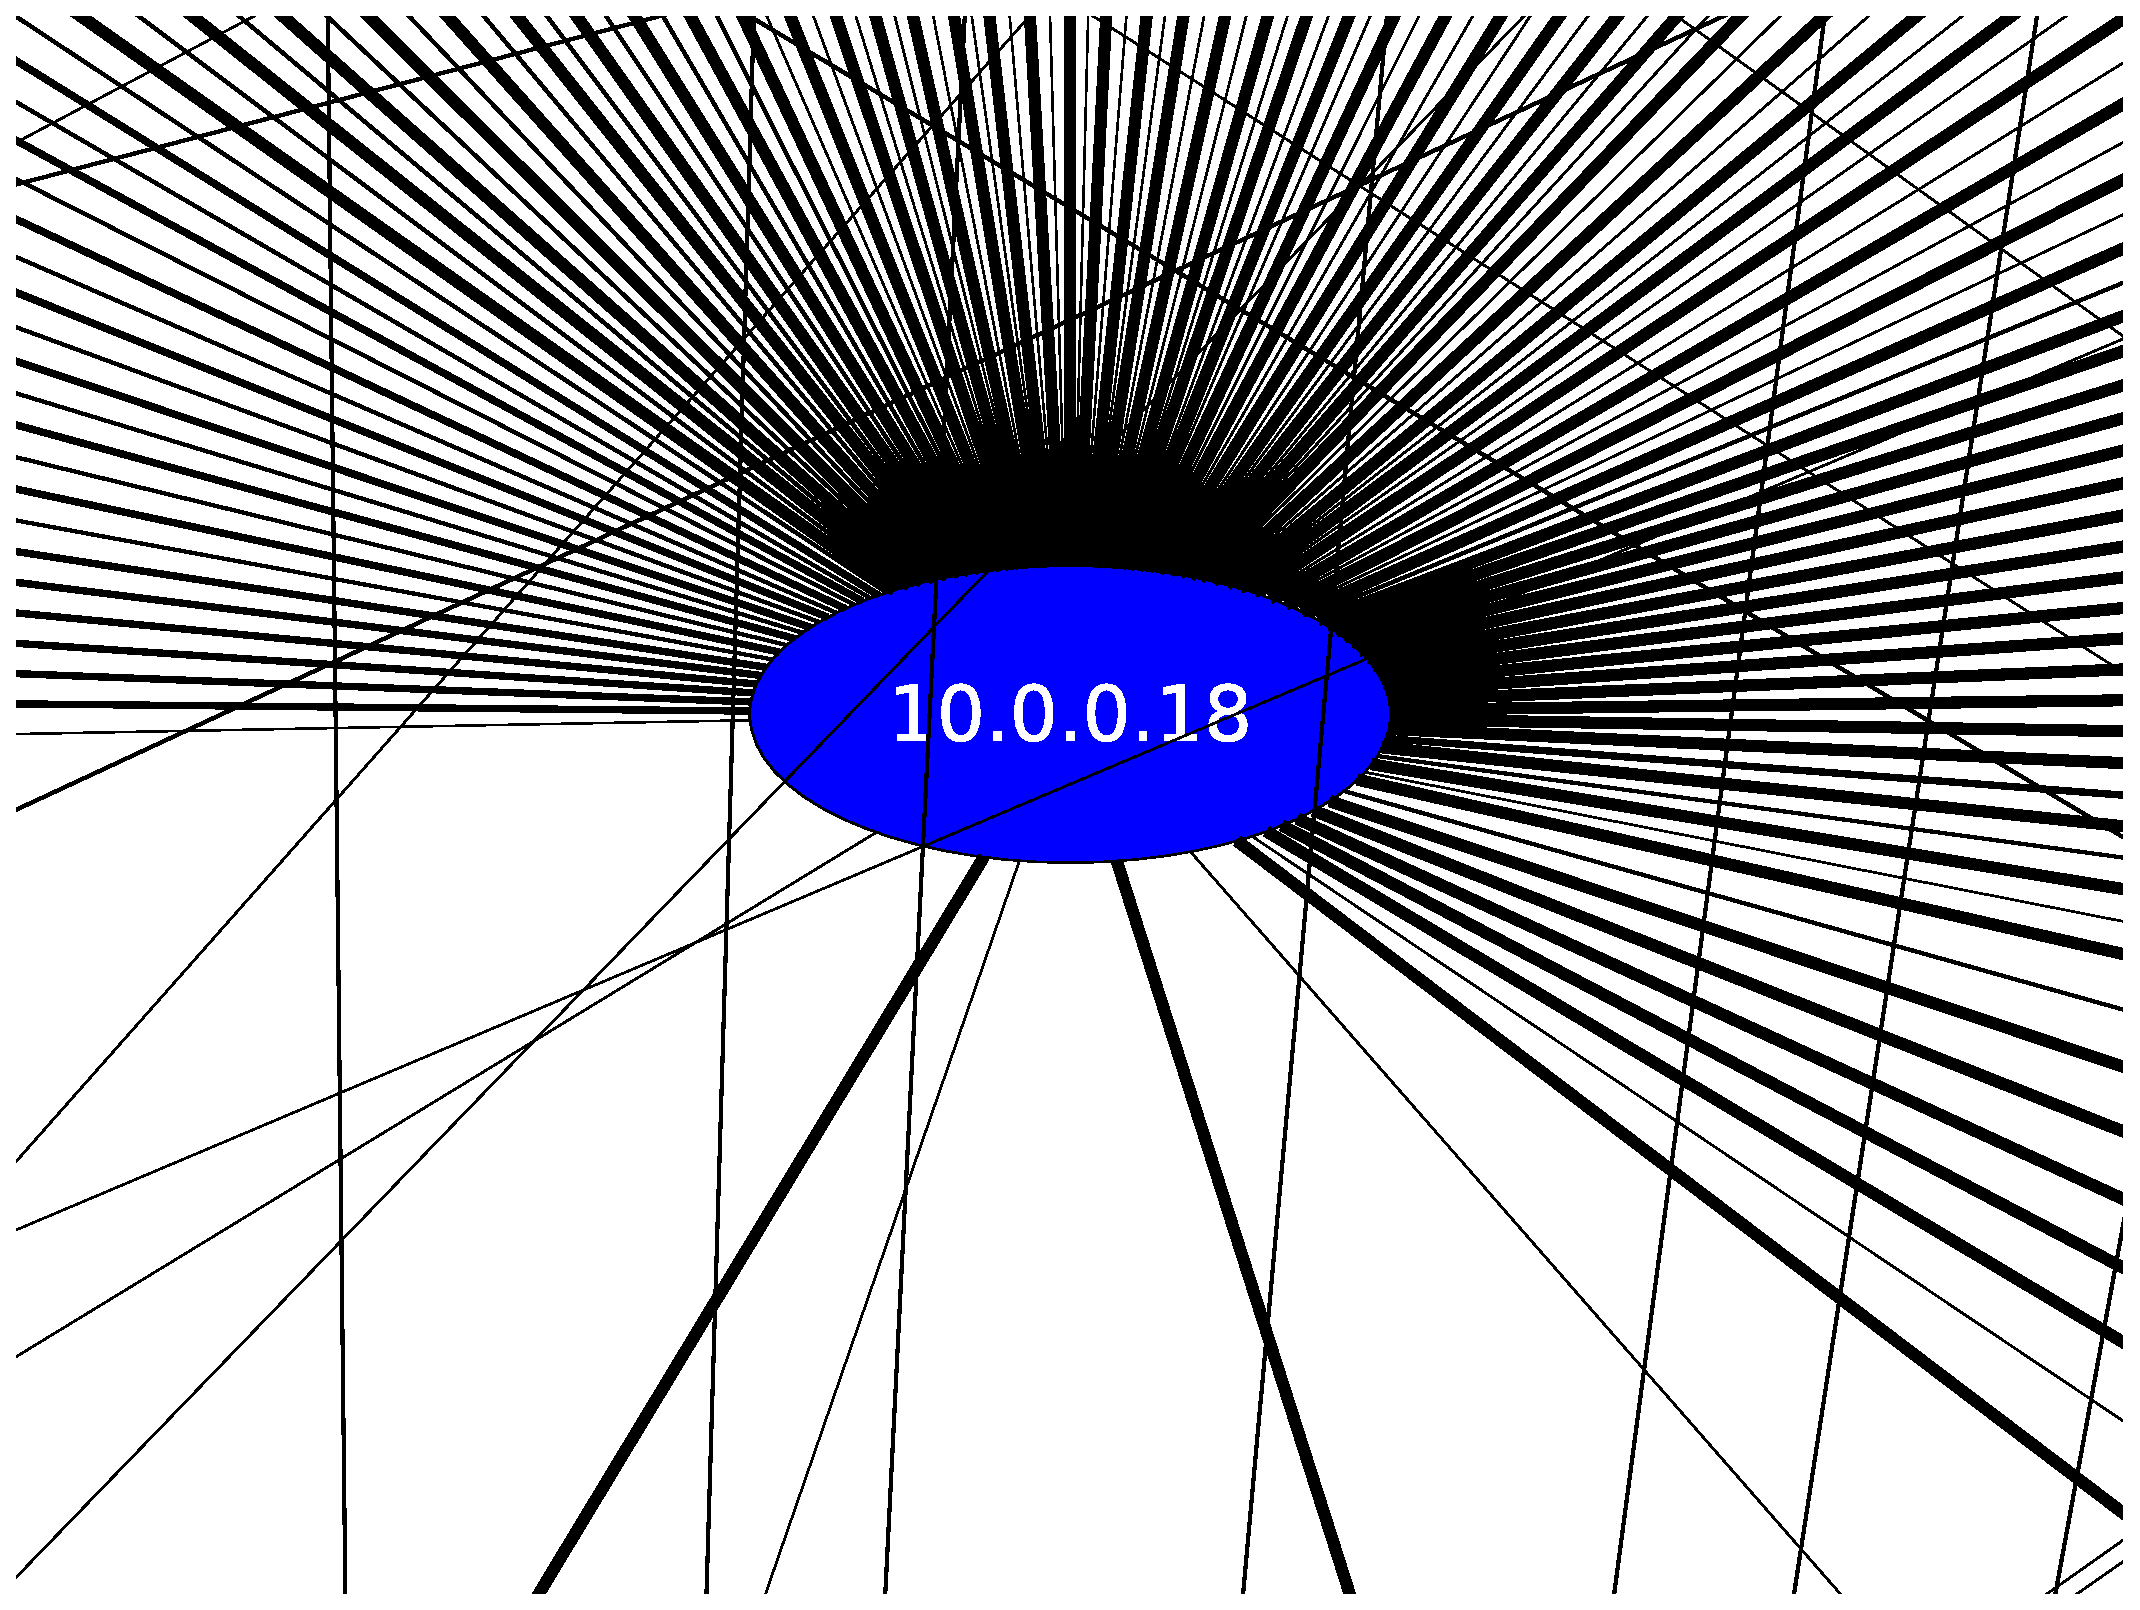
\includegraphics[width=0.5\textwidth]{img/graph/escenario_1/vlan1/vlan1_1000toEnd_10_0_0_18}
    \caption{VLAN \nameref{itm:vlan1} - 10.0.0.18}
    \label{fig:vlan1_grafo_10_0_0_18}
\end{figure}

\begin{figure}[!ht]
    \centering
    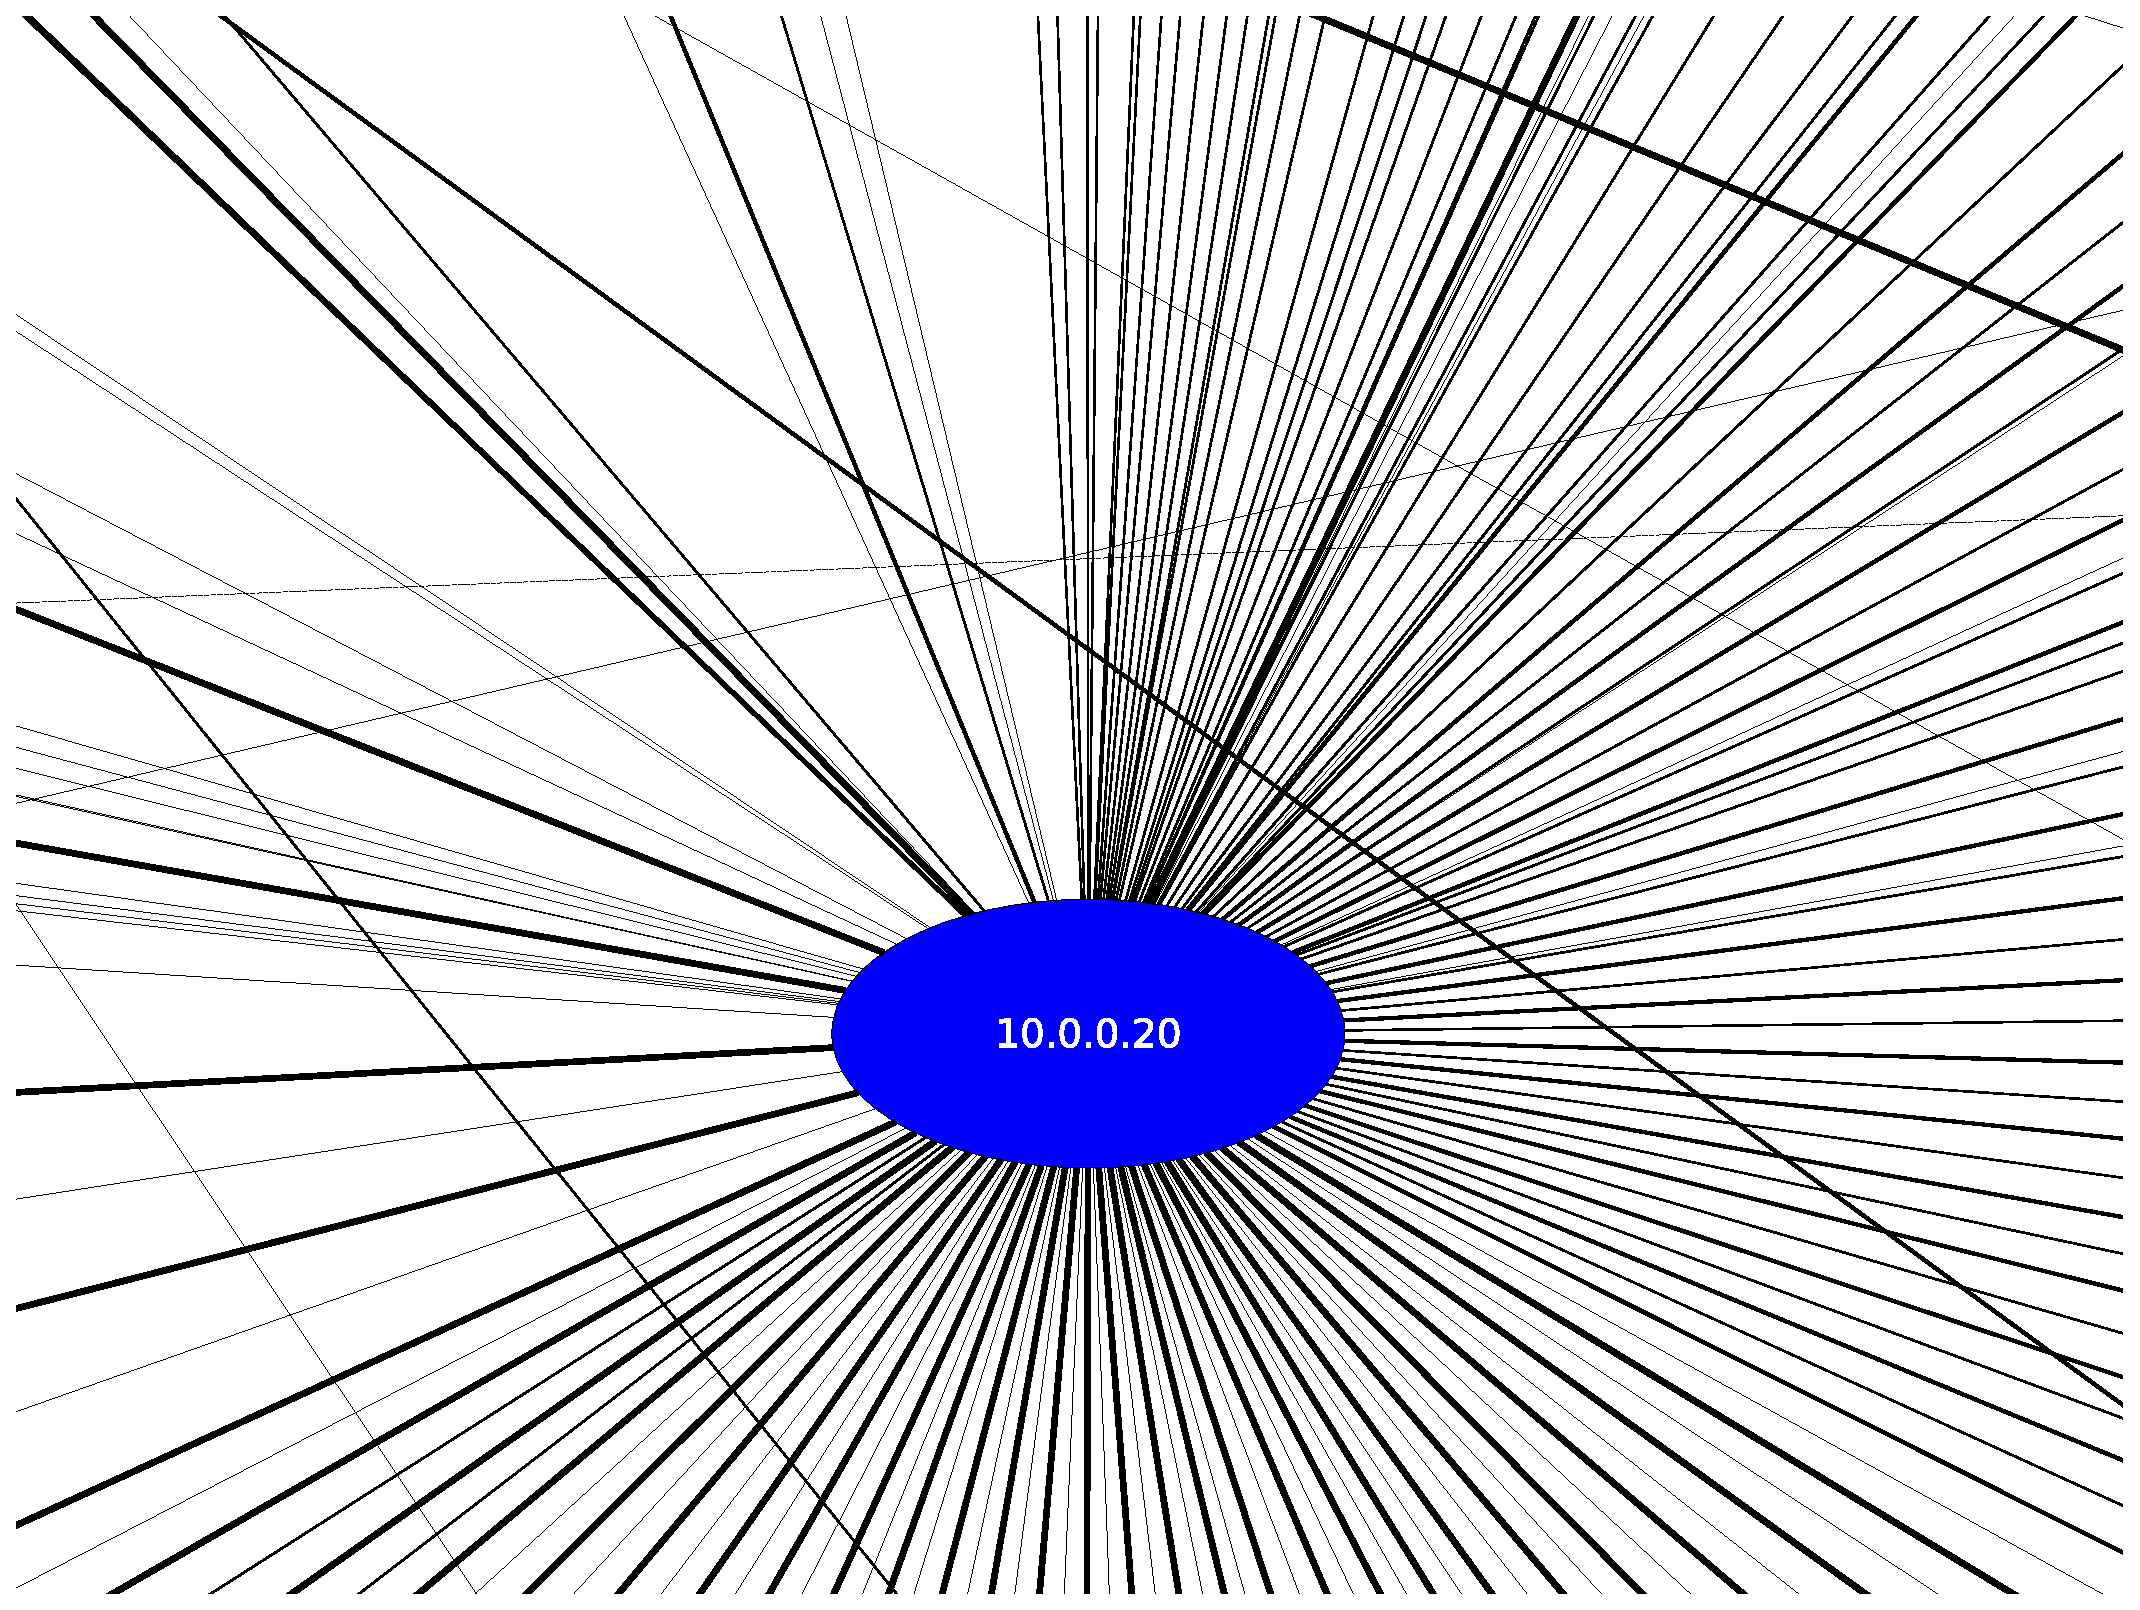
\includegraphics[width=0.5\textwidth]{img/graph/escenario_1/vlan1/vlan1_1000toEnd_10_0_0_20}
    \caption{VLAN \nameref{itm:vlan1} - 10.0.0.20}
    \label{fig:vlan1_grafo_10_0_0_20}
\end{figure}

\par Nos posicionamos ahora sobre la figura \ref{fig:vlan1_grafo_10_2_1_51}, donde se puede
ver que el nodo central no es un nodo azul ni rojo (aquellos nodos marcados por tener una
alta probabilidad en alguna de las dos fuentes de informaci\'on). Aqu\'i se puede observar dicho
host no solo recibe peticiones ARP de sus nodos circundantes, sino que tambi\'en env\'ia \'el
mismo sus propios paquetes del protocolo. As\'i pues, observamos que los nodos que lo rodean
tampoco tienen una gran interacci\'on, salvo alguna excepcion, con el resto de los nodos
\textit{alejados} de la red\footnote{El concepto de \textit{cercan\'ia} es meramente gr\'afico,
e incluso por ah\'i puede aplicar a la red, ya que claramente estos nodos env\'ian paquetes
ARP a el nodo central con frecuencia considerable y no as\'i a otras direcciones \textit{alejadas}
de la red.}. As\'i pues, podemos suponer que esta IP se encarga de ofrecerle alg\'un tipo
de servicio a las terminales que tratan de resolver su \textit{MAC}.

\par Siguiendo en esta figura, se observan las IPs \textit{10.1.254.1, 10.2.13.202 y
10.1.97.101} reciben mayormente conexiones de los nodos de menor tama\~no de esta figura.
Se podr\'ia llegar a suponer que estas direcciones son pose\'idas por hosts que ofrecen
alg\'un tipo de servicio que no requiera ser iniciado por ellos mismos, como por ejemplo,
una base de datos.

\begin{figure}[!htb]
    \centering
    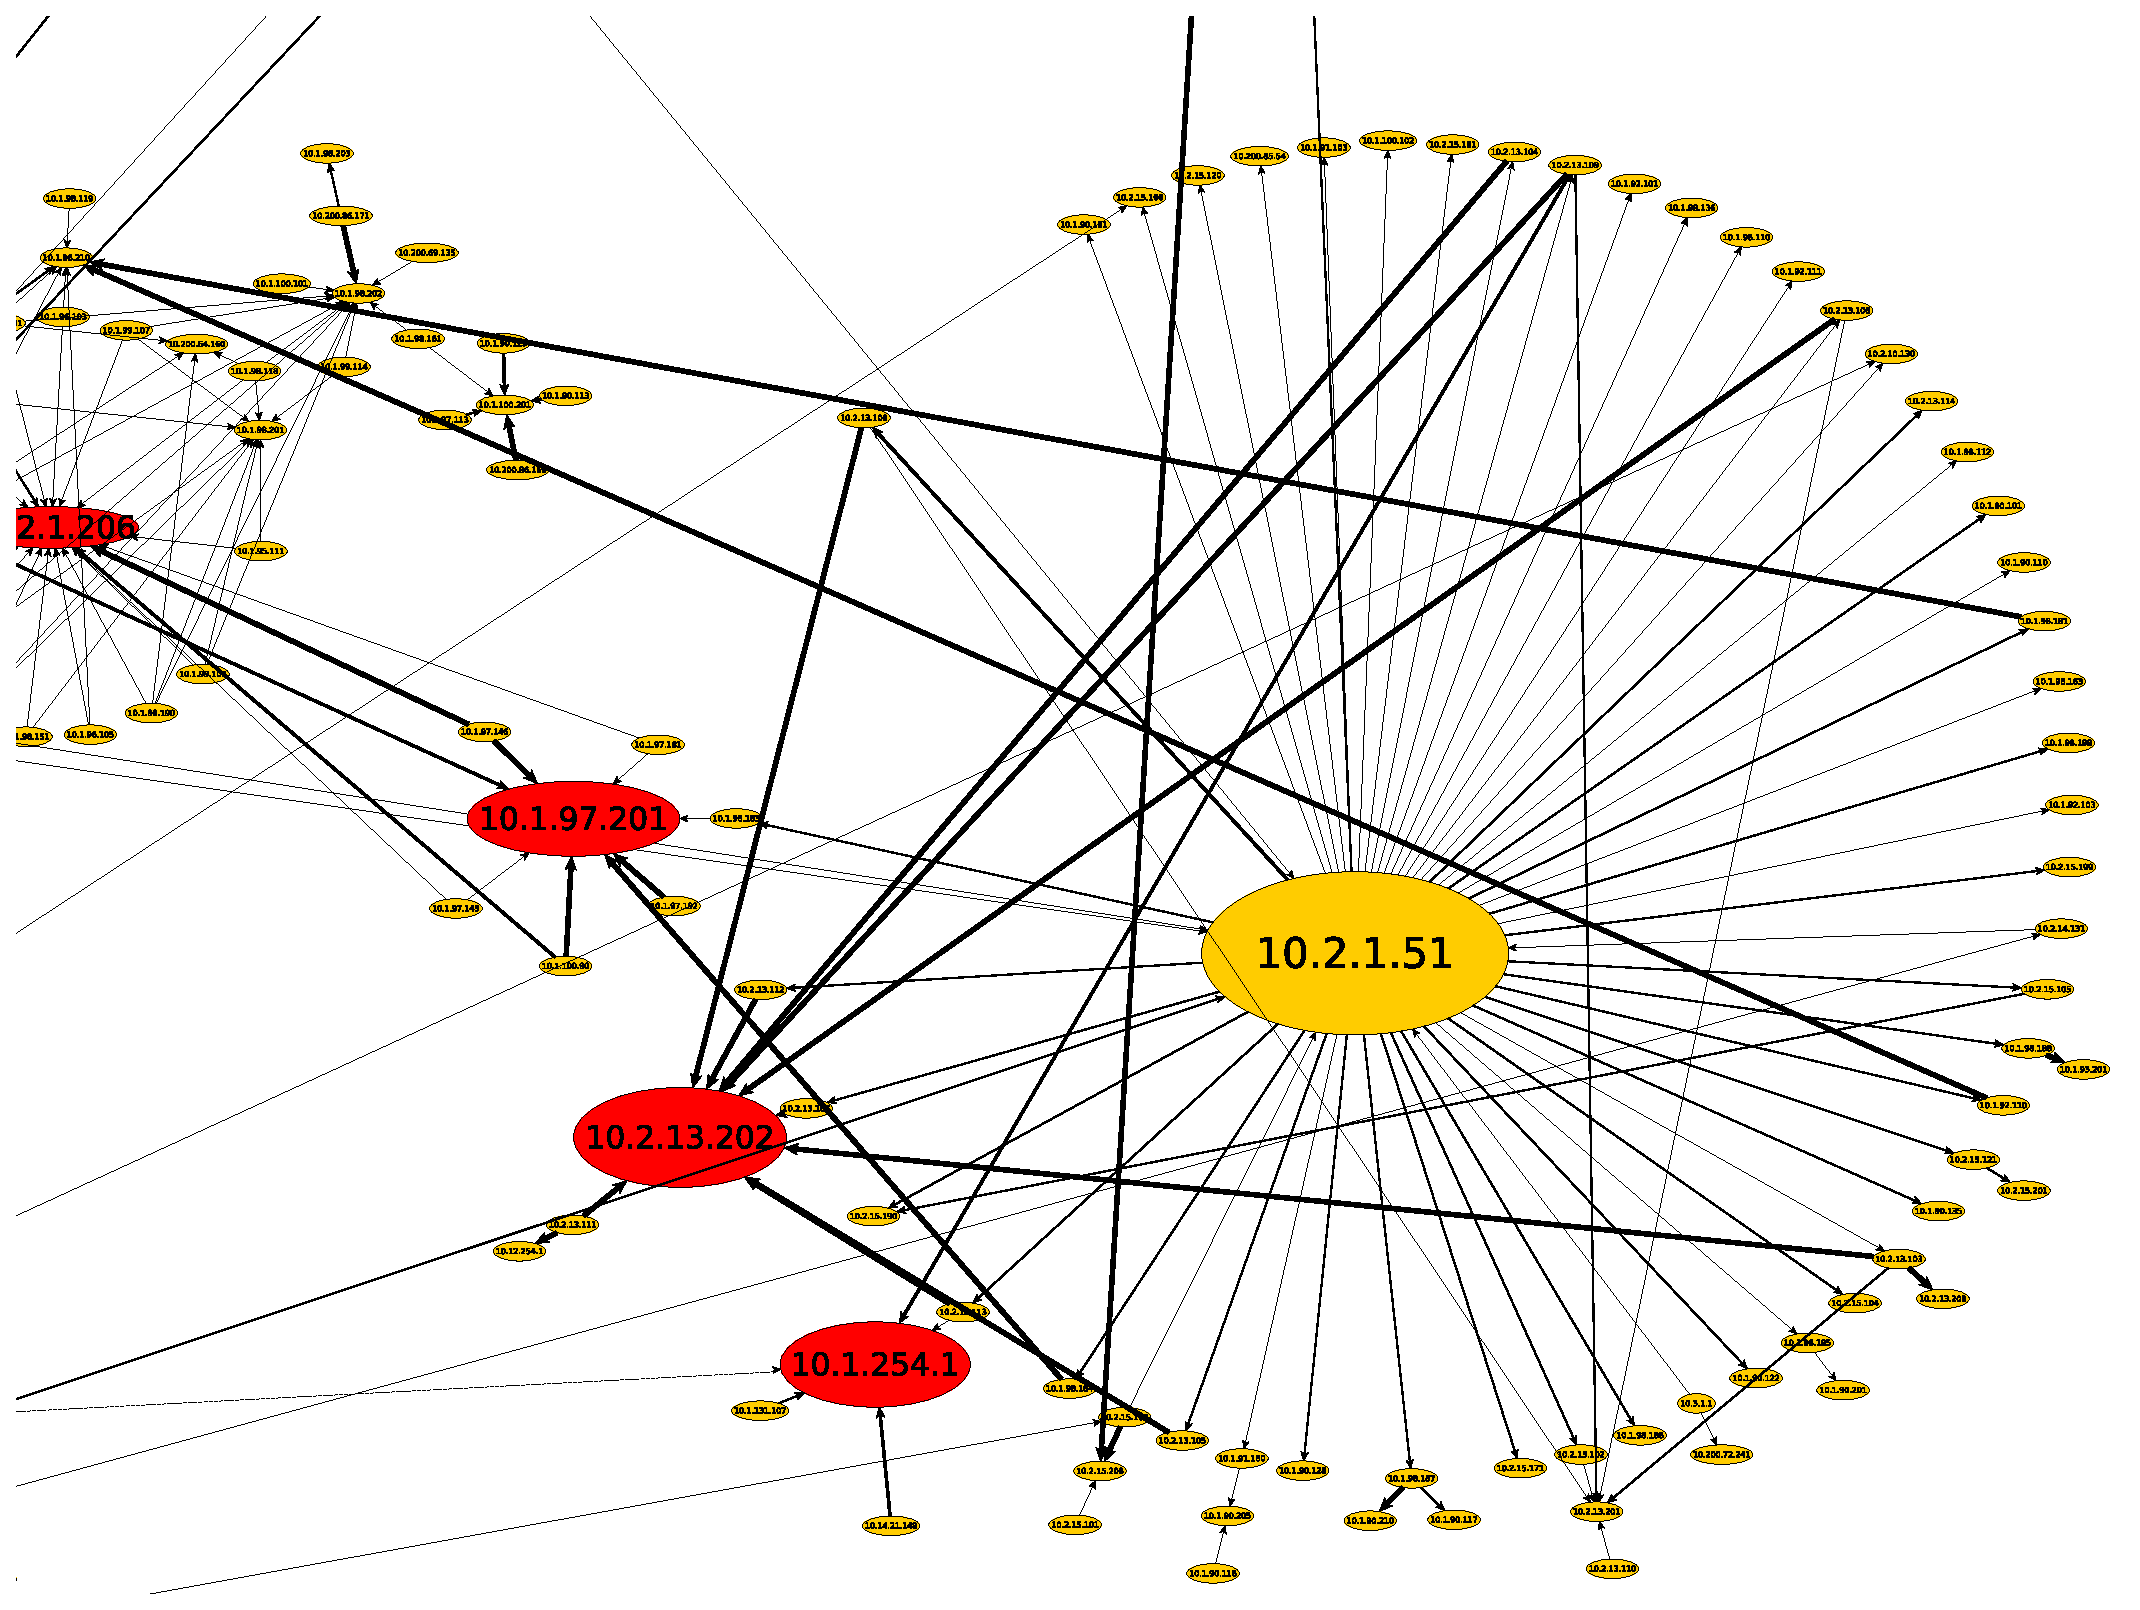
\includegraphics[width=0.5\textwidth]{img/graph/escenario_1/vlan1/vlan1_1000toEnd_10_2_1_51}
    \caption{VLAN \nameref{itm:vlan1} - 10.2.1.51}
    \label{fig:vlan1_grafo_10_2_1_51}
\end{figure}

\par En la misma l\'inea, se aplica lo reci\'en dicho a las figuras \ref{fig:vlan1_grafo_10_2_1_206},
\ref{fig:vlan1_grafo_10_1_254_5} y \ref{fig:vlan1_grafo_10_200_0_44} donde se obserba
el mismo tipo de grafo y comportamiento.

\begin{figure}[!htb]
    \centering
    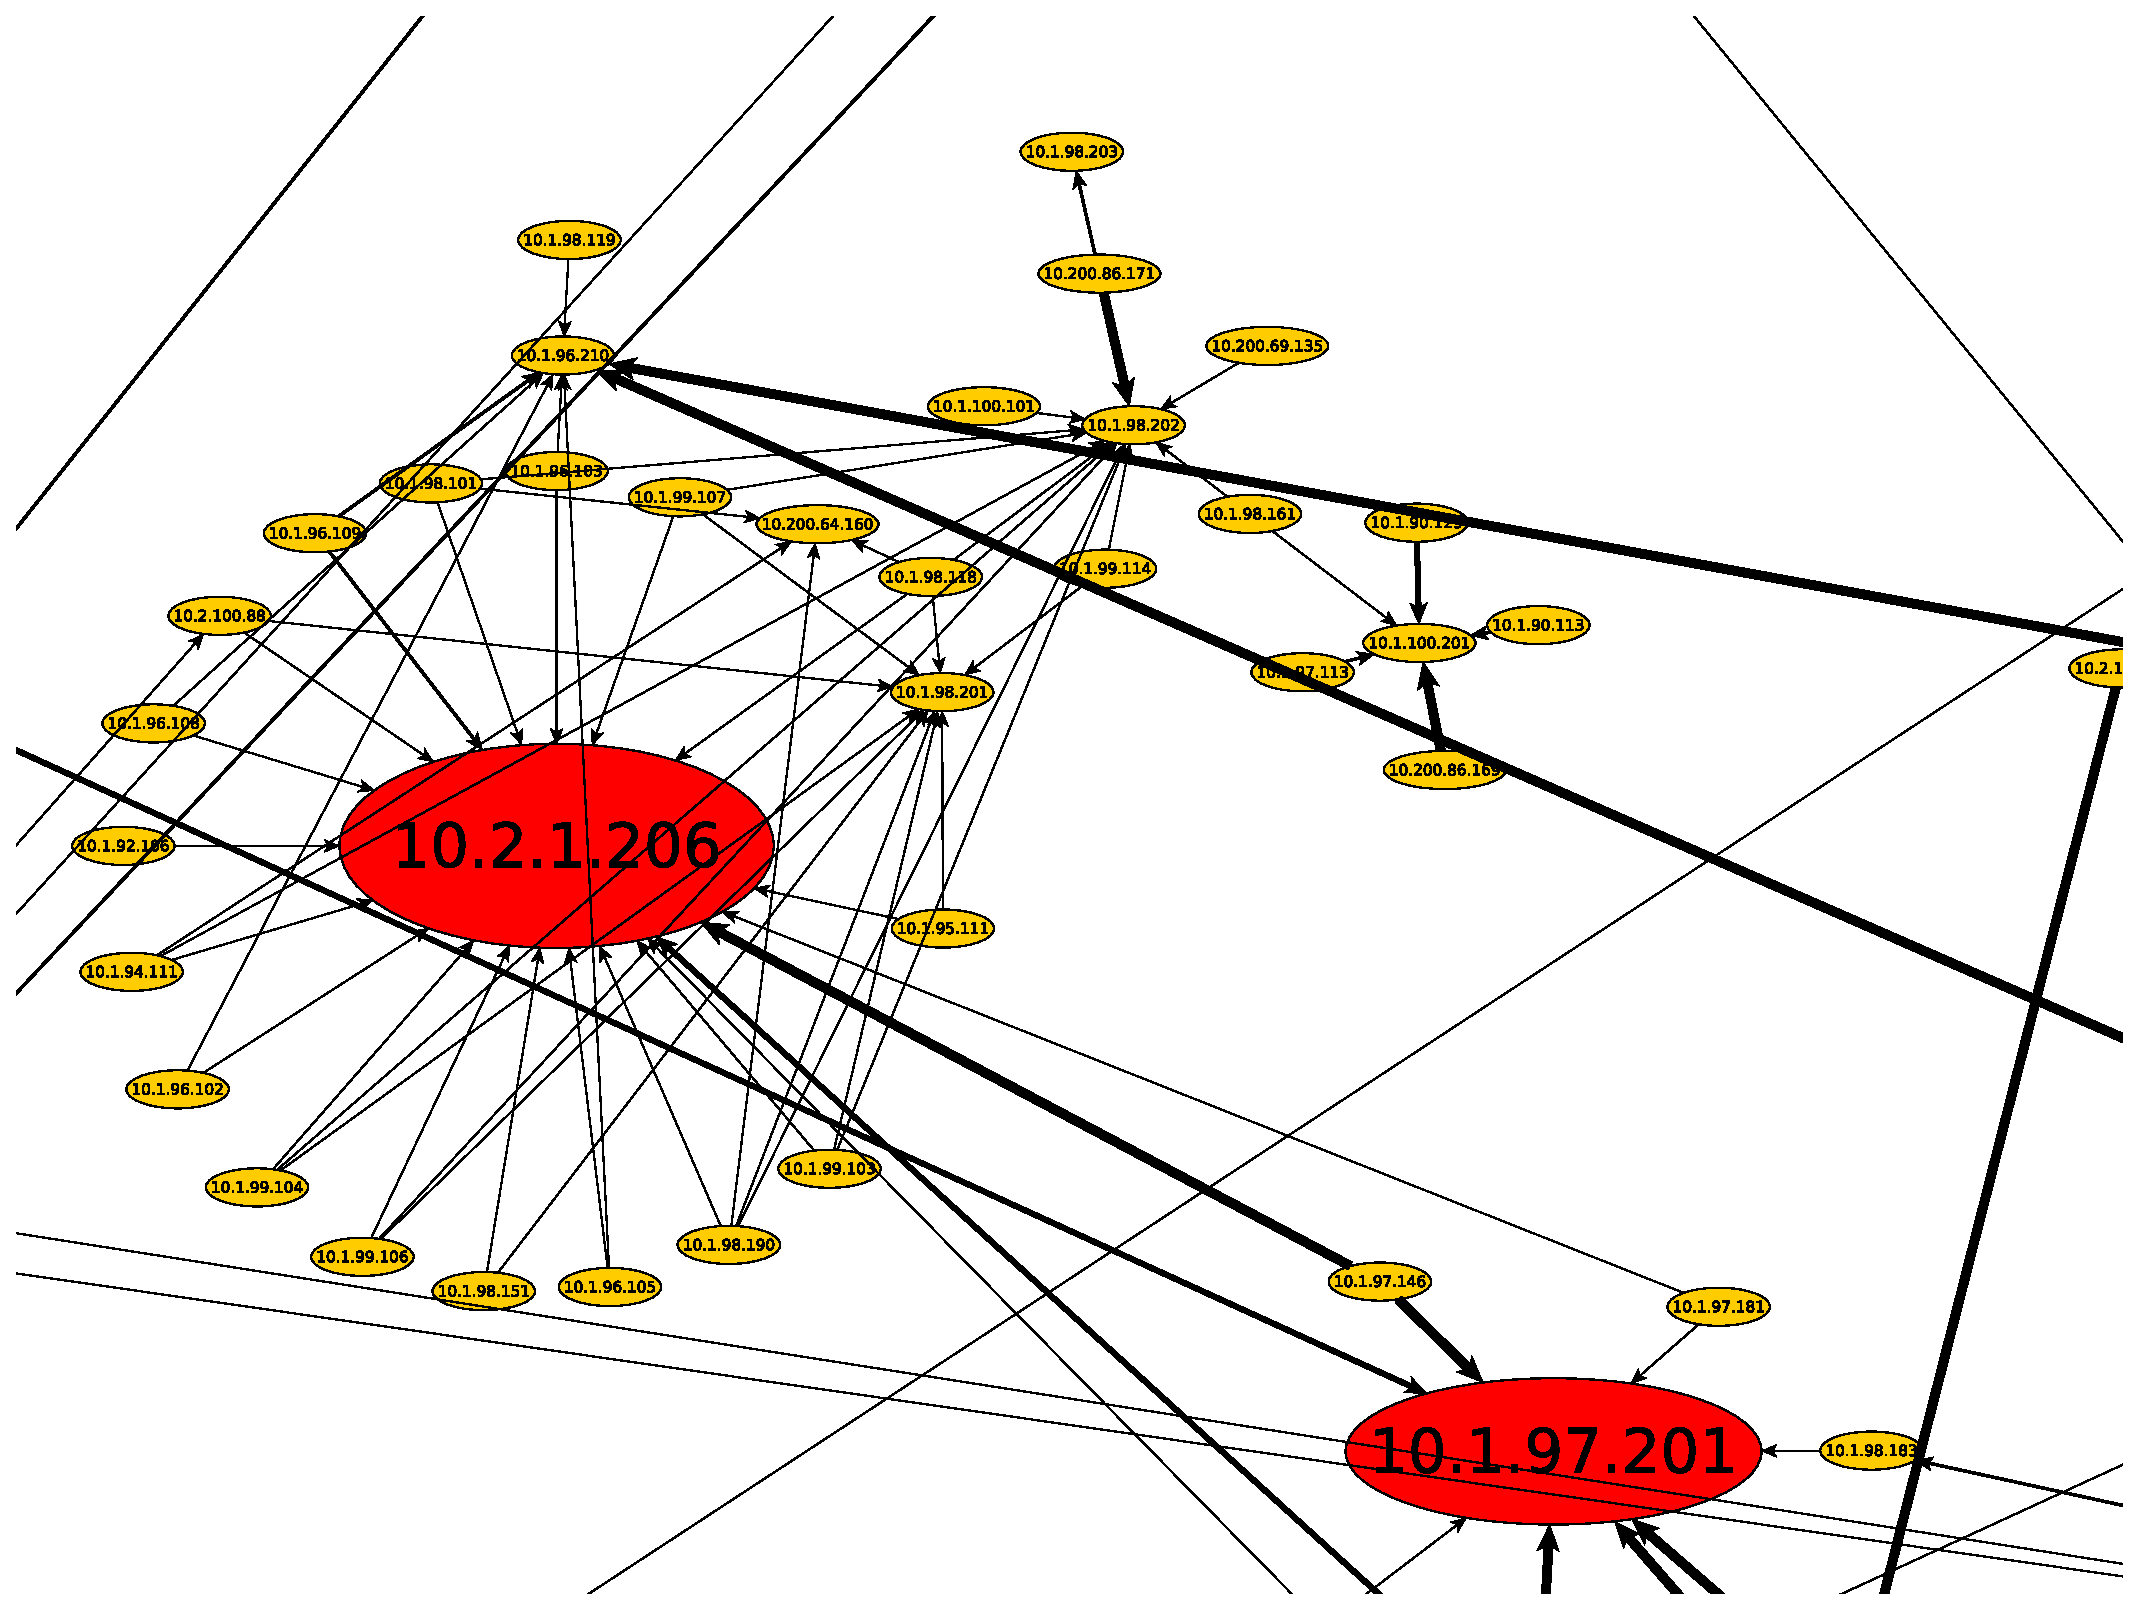
\includegraphics[width=0.5\textwidth]{img/graph/escenario_1/vlan1/vlan1_1000toEnd_10_2_1_206}
    \caption{VLAN \nameref{itm:vlan1} - 10.2.1.206}
    \label{fig:vlan1_grafo_10_2_1_206}
\end{figure}

\begin{figure*}
    \centering
    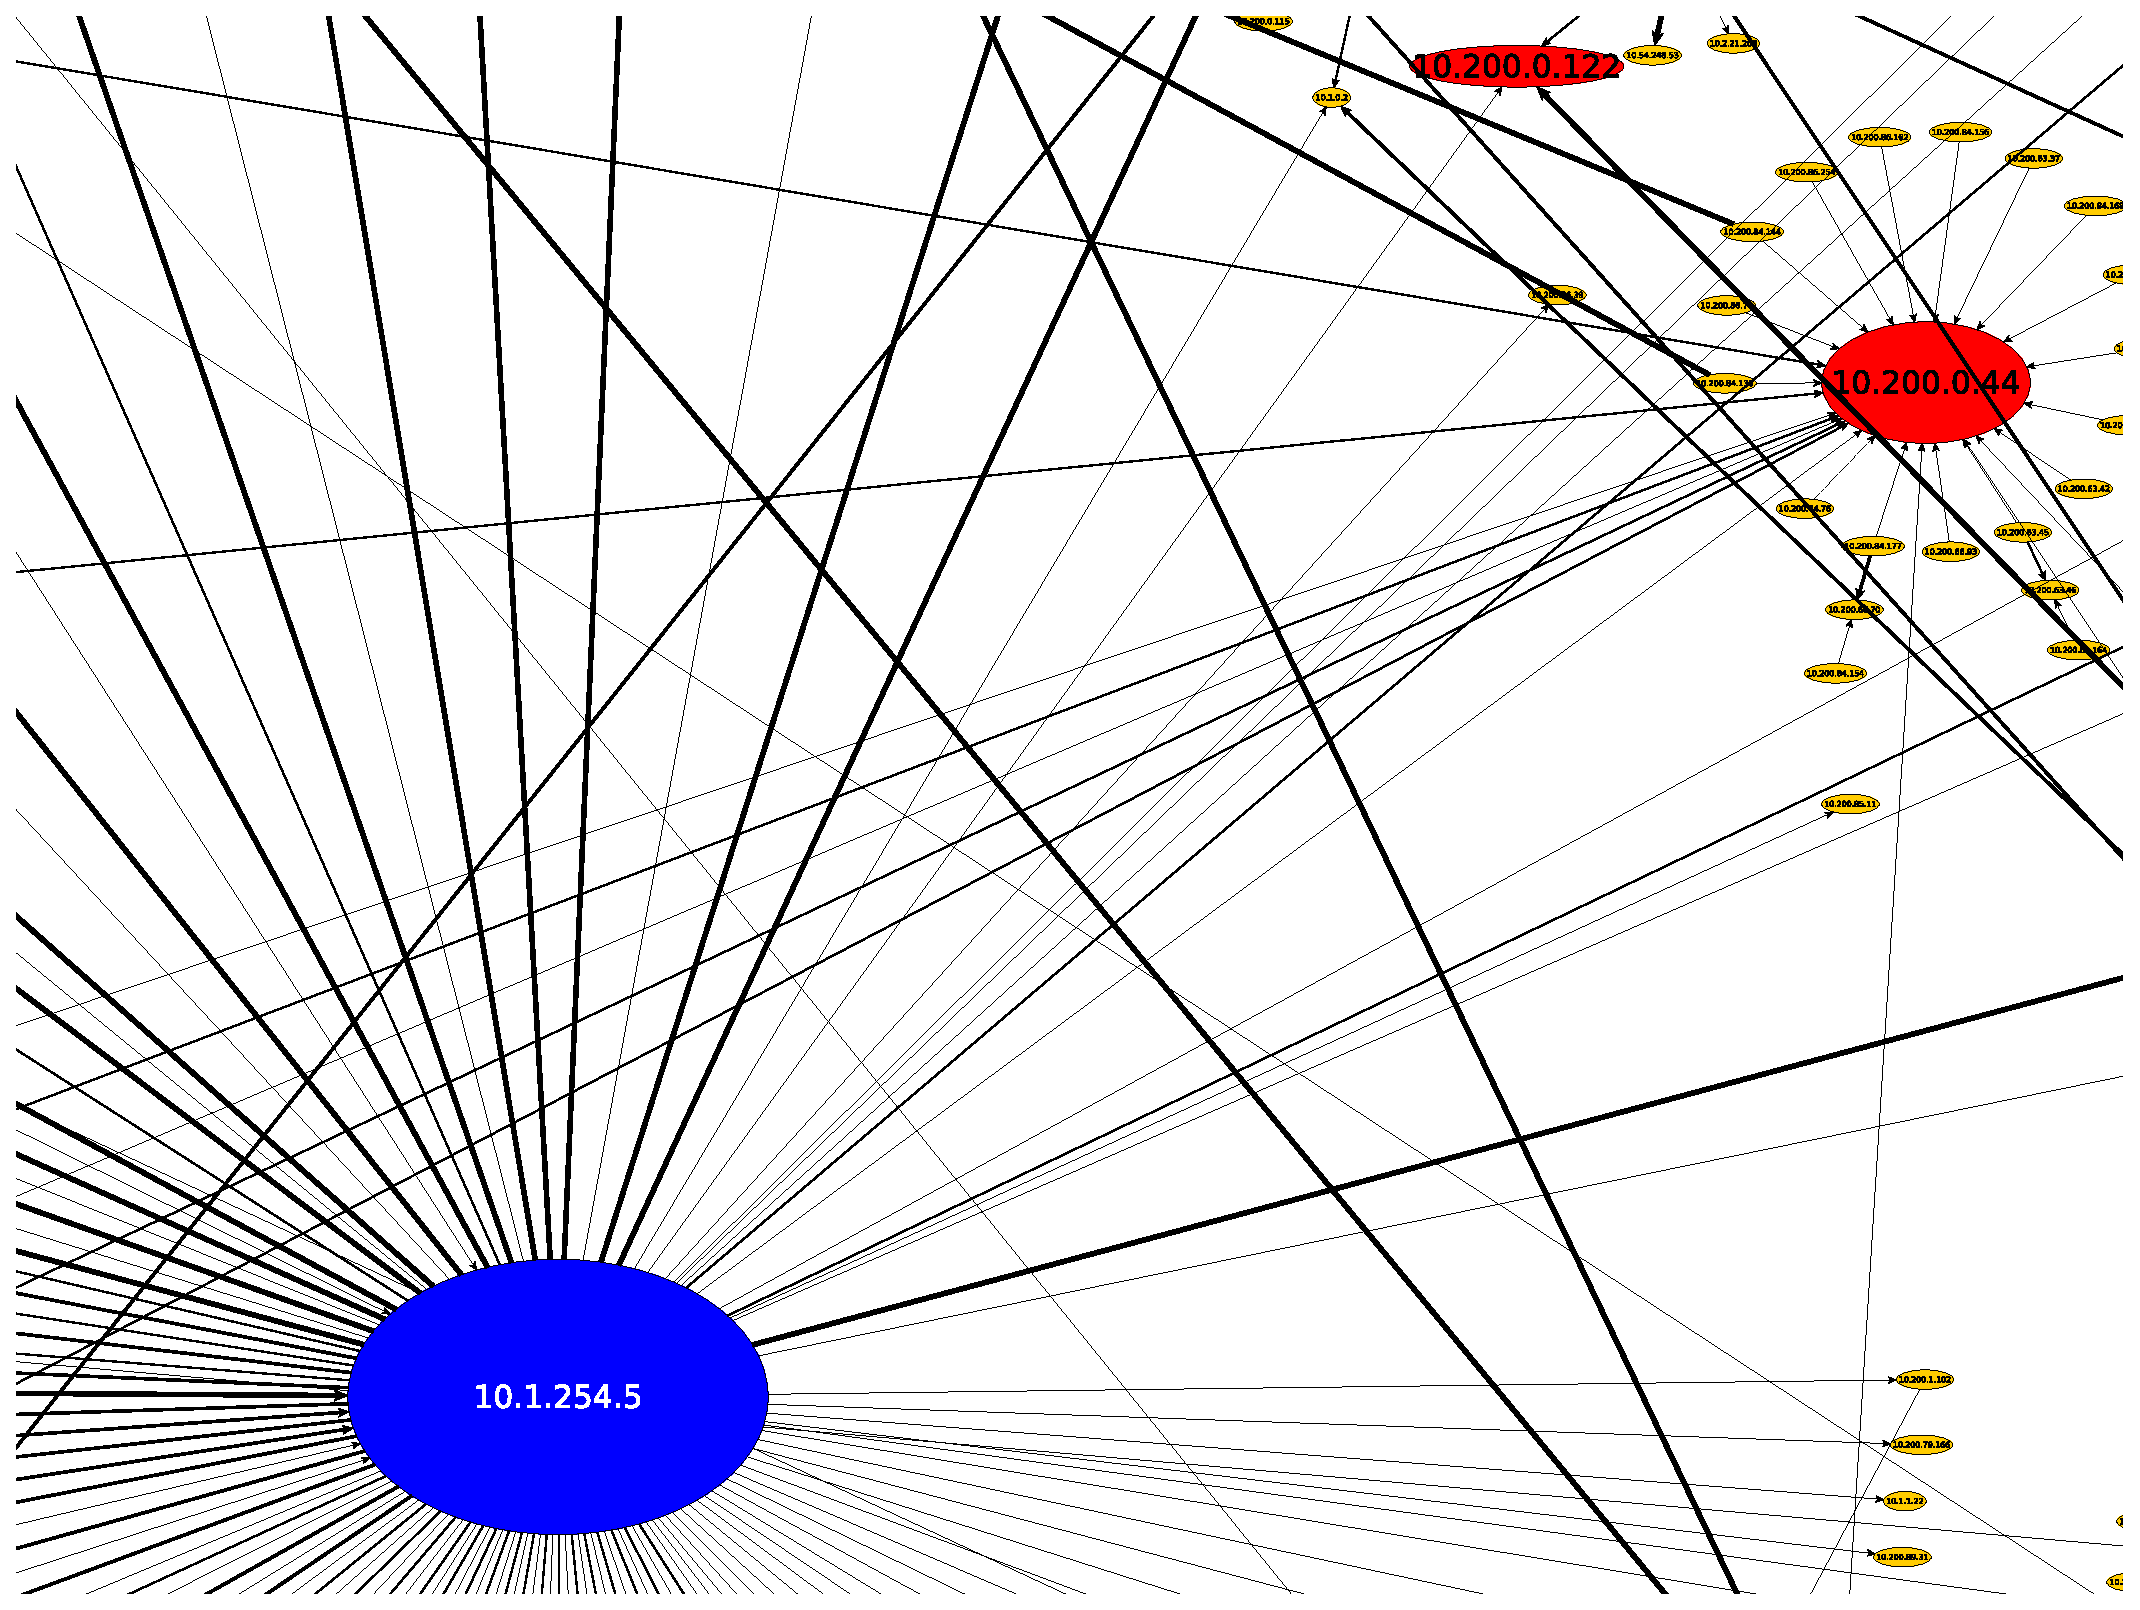
\includegraphics[width=\textwidth]{img/graph/escenario_1/vlan1/vlan1_1000toEnd_10_1_254_5}
    \caption{VLAN \nameref{itm:vlan1} - 10.1.254.5}
    \label{fig:vlan1_grafo_10_1_254_5}
\end{figure*}

\begin{figure}[!ht]
    \centering
    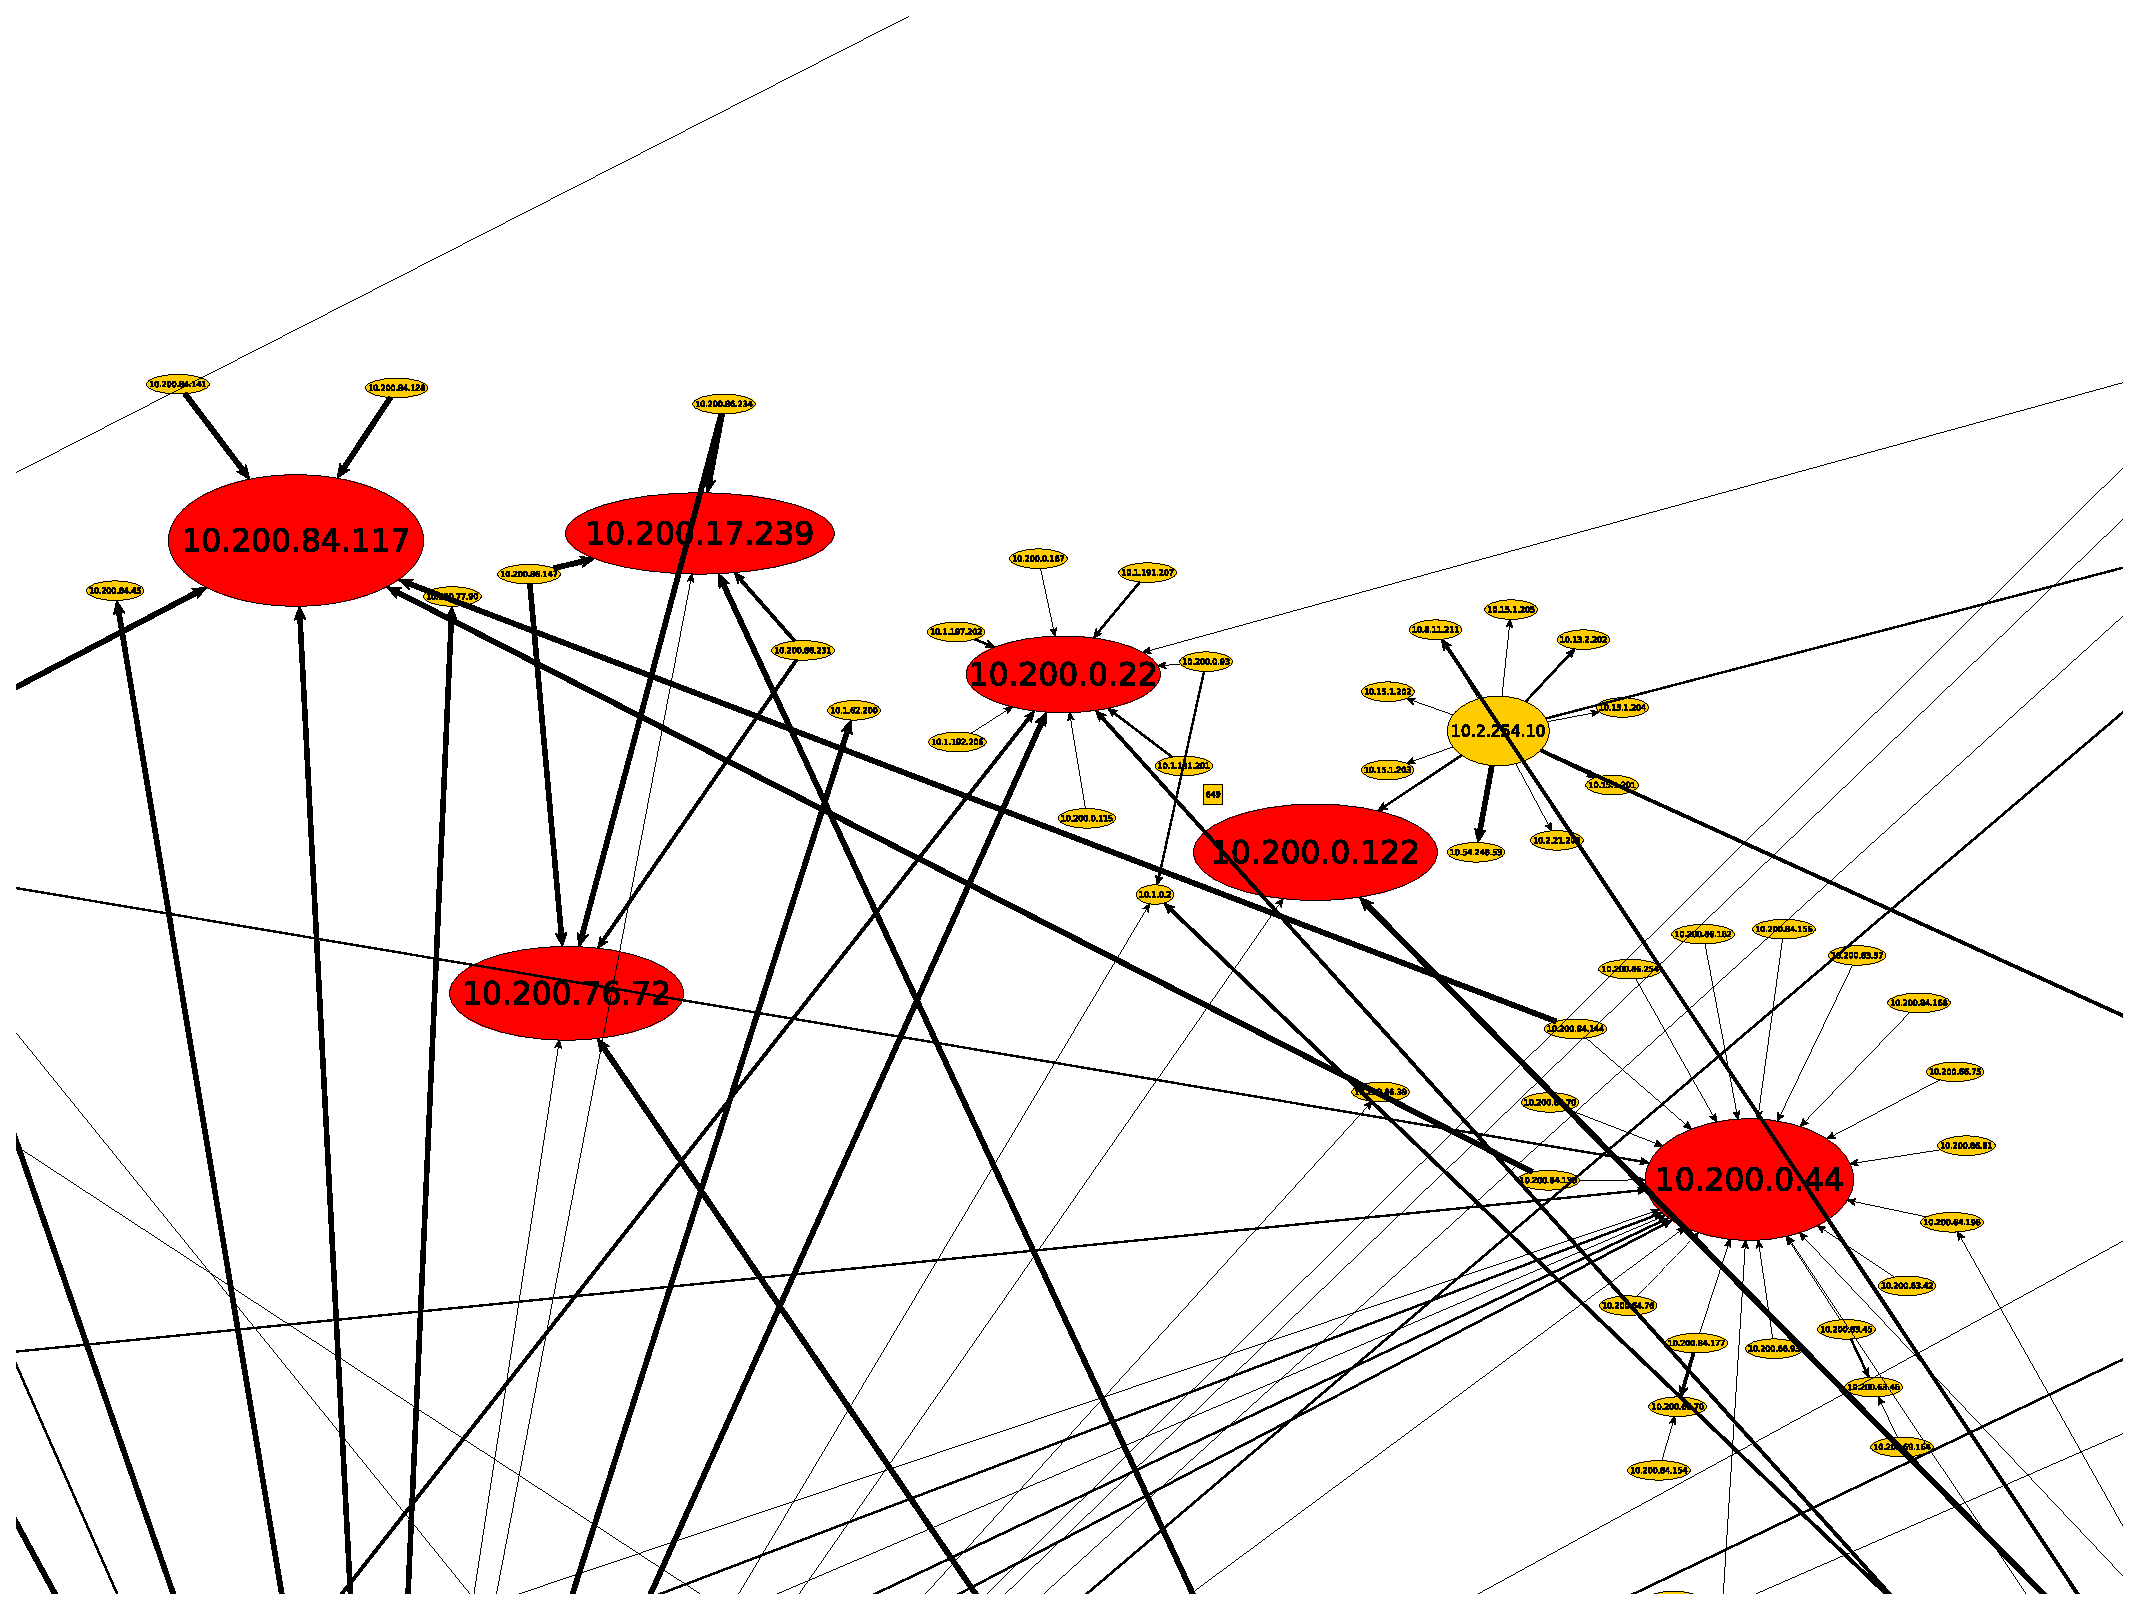
\includegraphics[width=0.5\textwidth]{img/graph/escenario_1/vlan1/vlan1_1000toEnd_10_200_0_44}
    \caption{VLAN \nameref{itm:vlan1} - 10.200.0.44}
    \label{fig:vlan1_grafo_10_200_0_44}
\end{figure}

\FloatBarrier
